\documentclass[12pt]{report}
\usepackage{graphicx} %required for everything 

%for wrapped figures 
\usepackage{wrapfig}

%for primitive graphic centering without a figure environment 
\usepackage[export]{adjustbox}

%for right-sided captions only 
\usepackage[rightcaption]{sidecap}

\usepackage{lipsum}

\graphicspath{{./}} %the path here will be the default directory that \includegraphics looks for

% If you have two files with the same name but one is png and one is pdf, this command tells it to use the png first. This is because it's typically cheaper to compile with the png. However, for better quality (like for publication), you would switch the order of the two extensions. 
% Images in vector form should be a pdf, and images in bitmap form should be in png or jpg 
\DeclareGraphicsExtensions{.jpg, .png,.pdf}
\begin{document}
\listoffigures %much like a TOC

\chapter{figures}
% 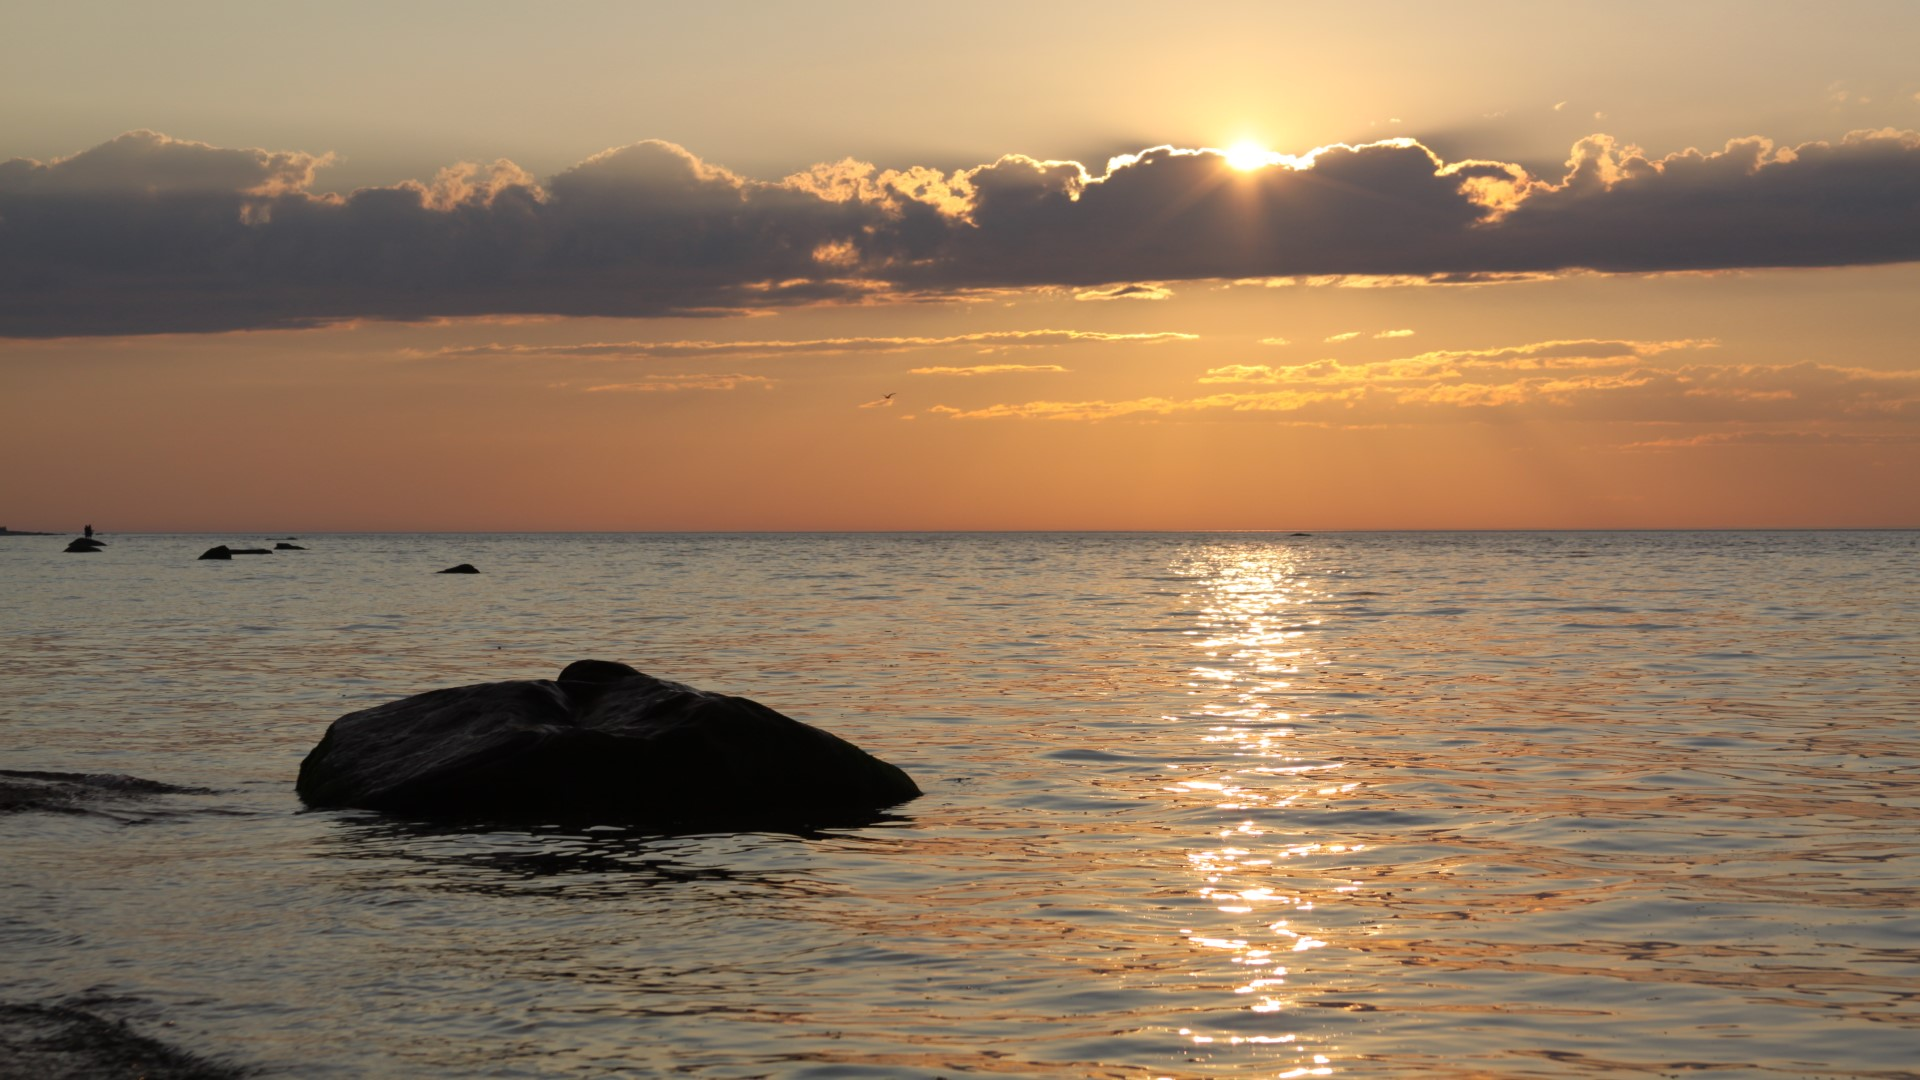
\includegraphics{demo.jpg}
\section{Simple figures}

%if you specify both heights and widths, it will artificially stretch. Specifying one parameter will scale the other one to keep the aspect ratio 
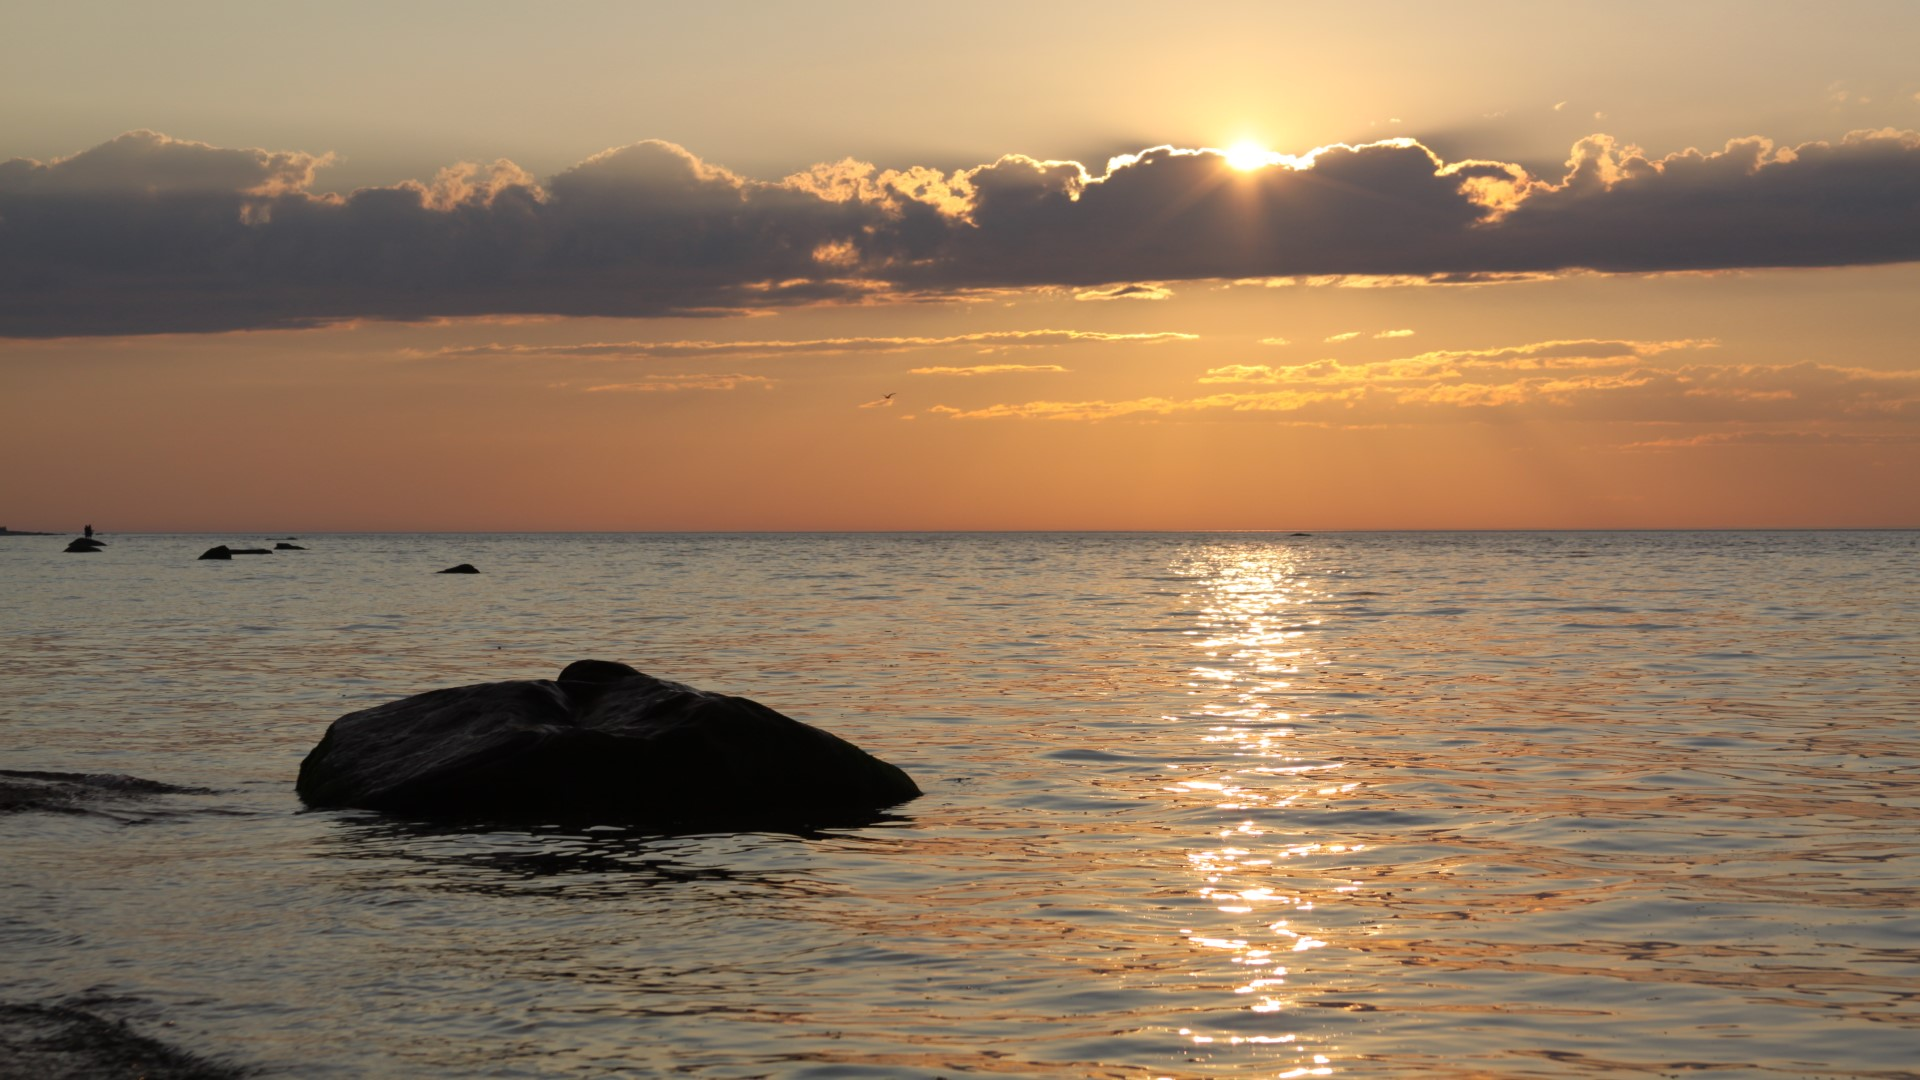
\includegraphics[height = 6cm, width = 0.5\textwidth]{demo} %suffix optional 

\vspace{2em}

%you can also use manual scaling, and you can even rotate 
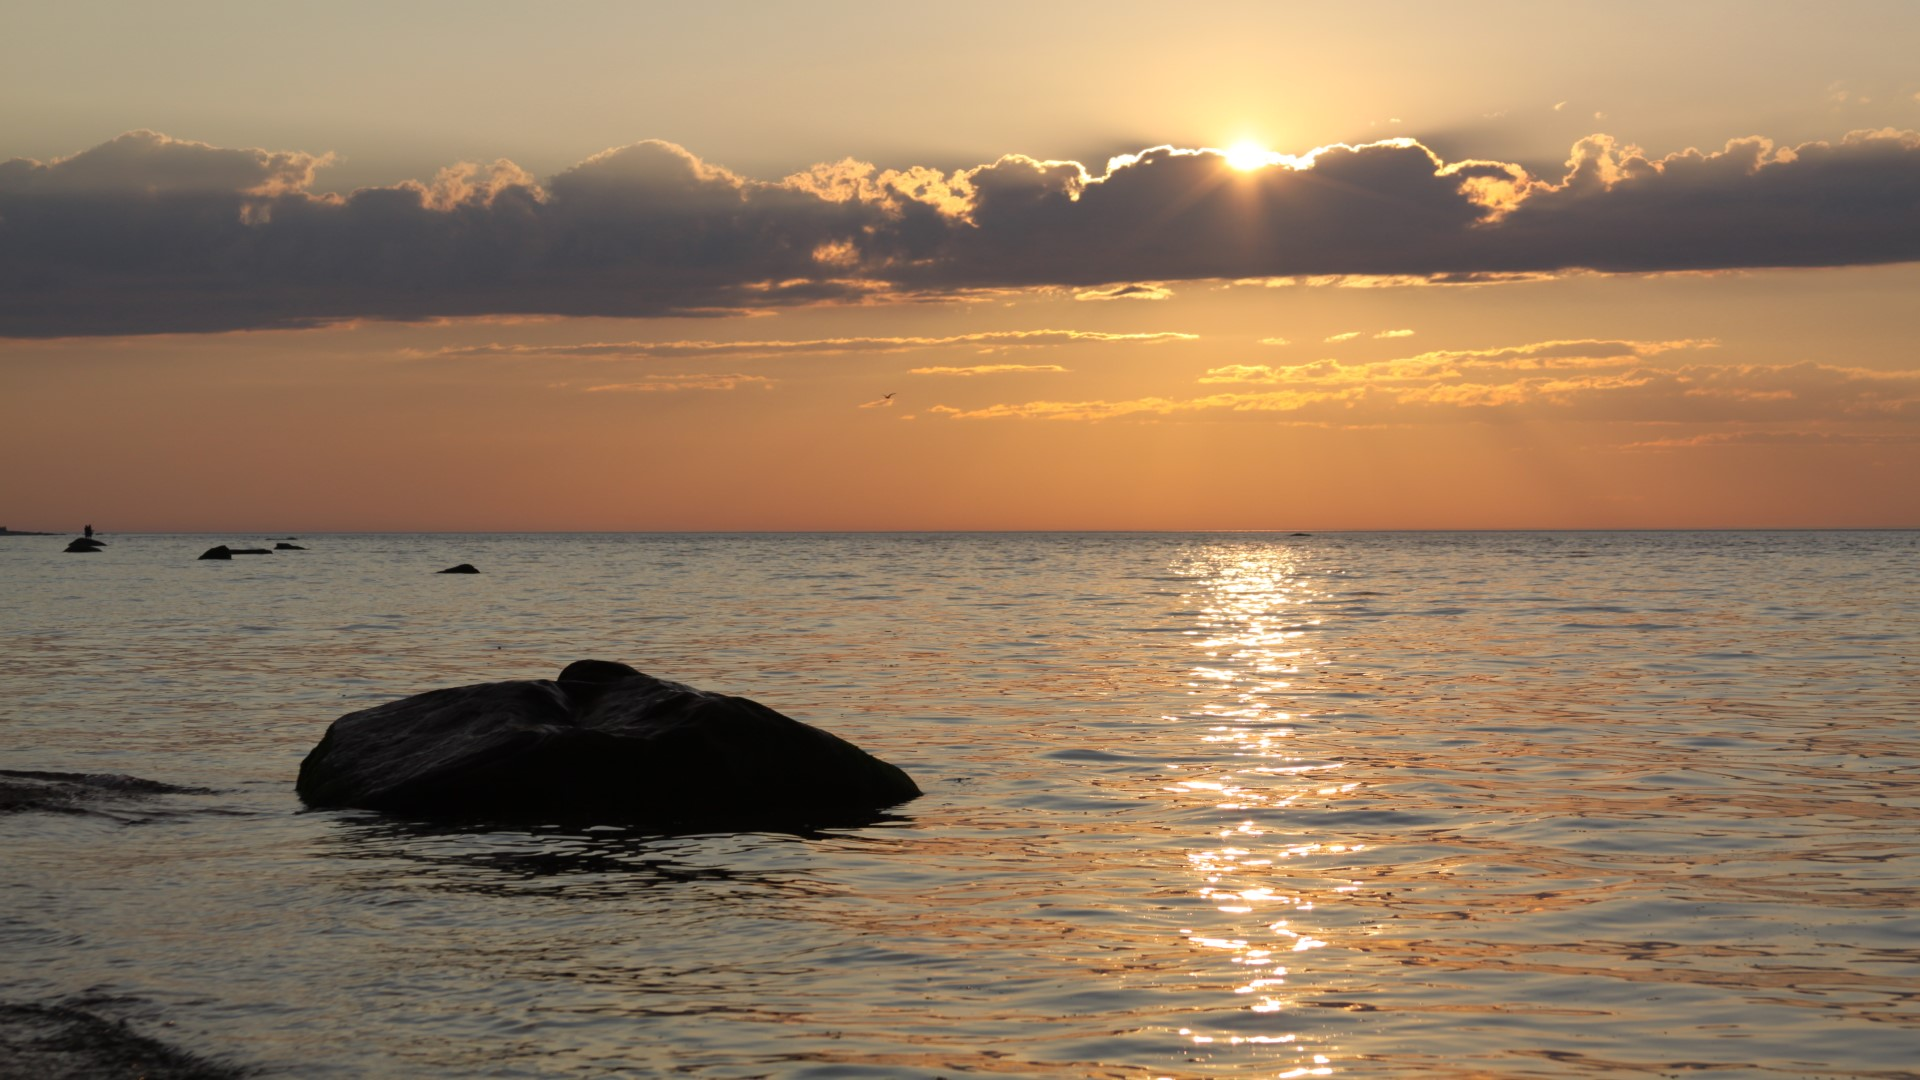
\includegraphics[scale = 0.1, angle = 45]{demo} 

%to do primitive alignment: 
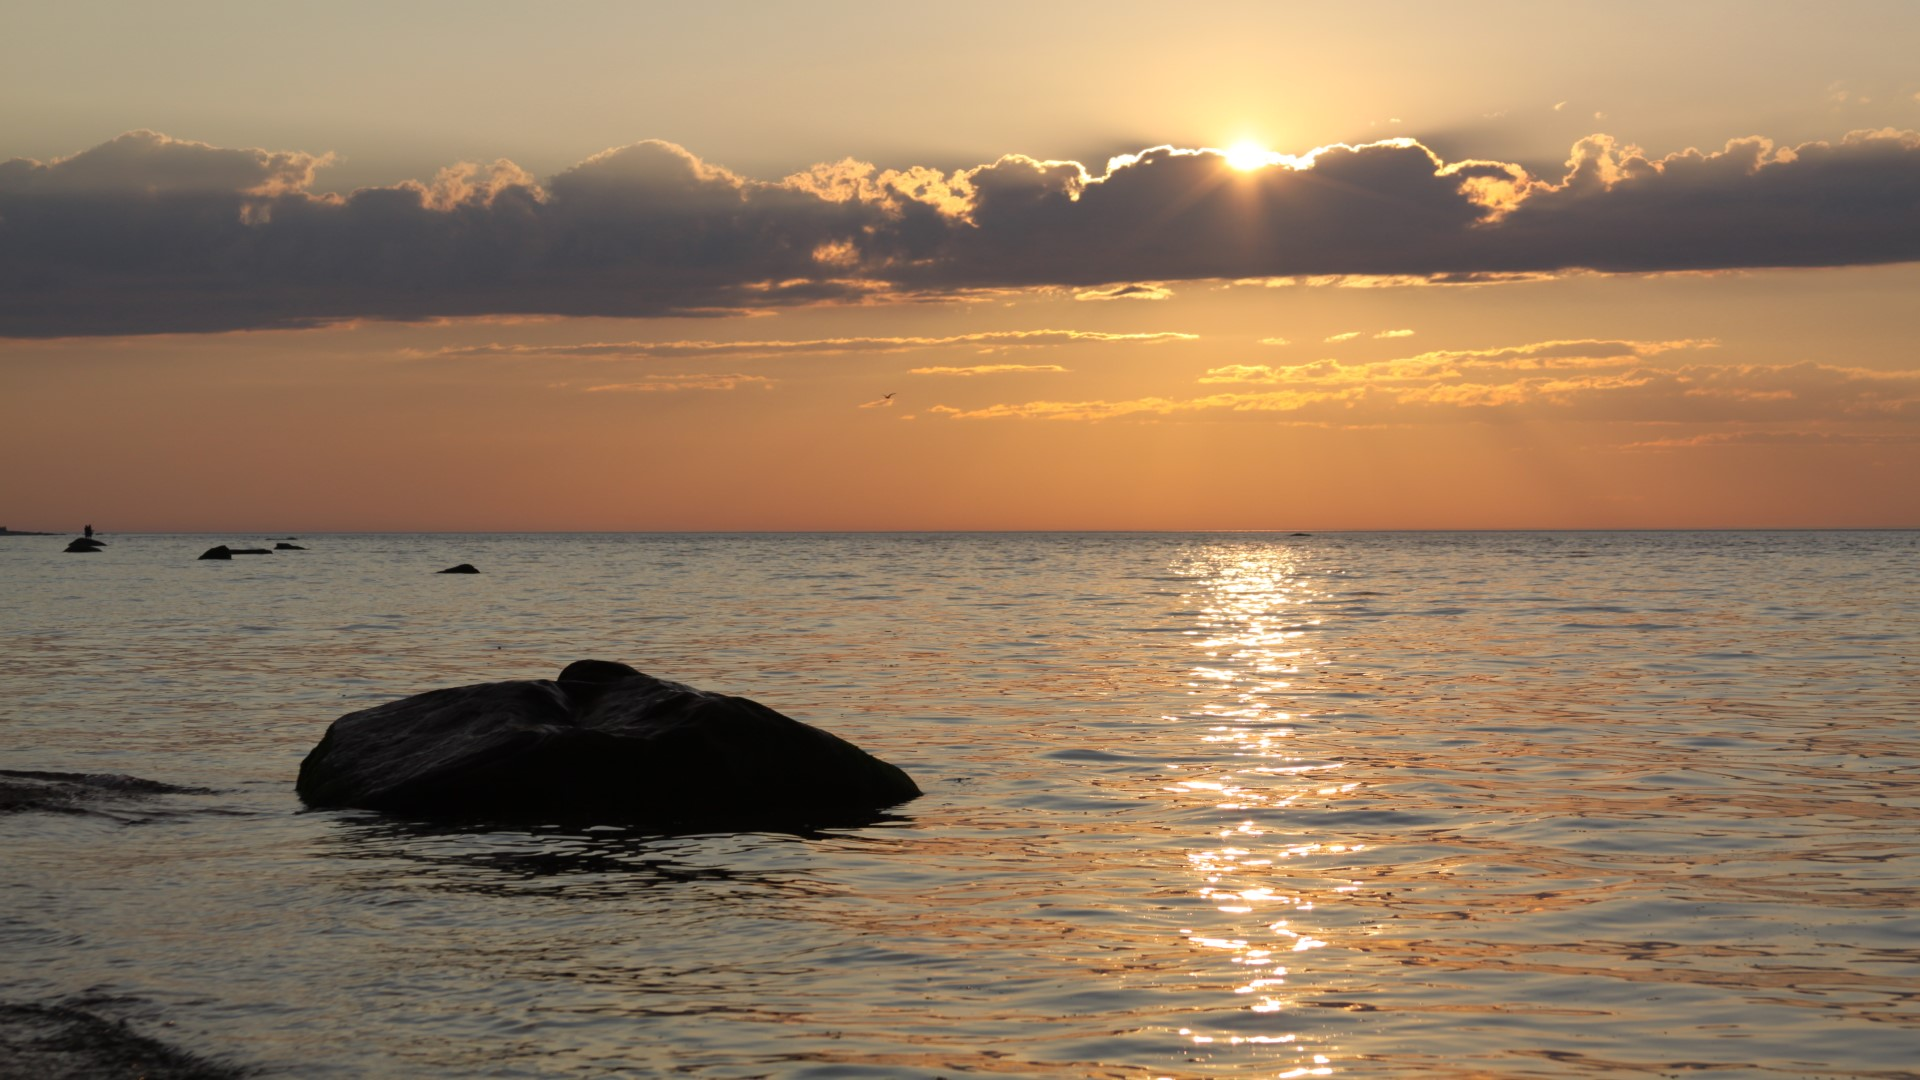
\includegraphics[width=0.5\textwidth, right]{demo} %left, right, center, inner, outer 

\section{Figure environment}
%this is a standard, vanilla figure environment. For most of your purposes, this is the only thing you need 
%h means here, t means top, b means bottom, p means special page, "!" suffix means force, and H means PLACE RIGHT HERE ( requires \usepackage{float})
\begin{figure}[h]
    \centering %centers everything 
    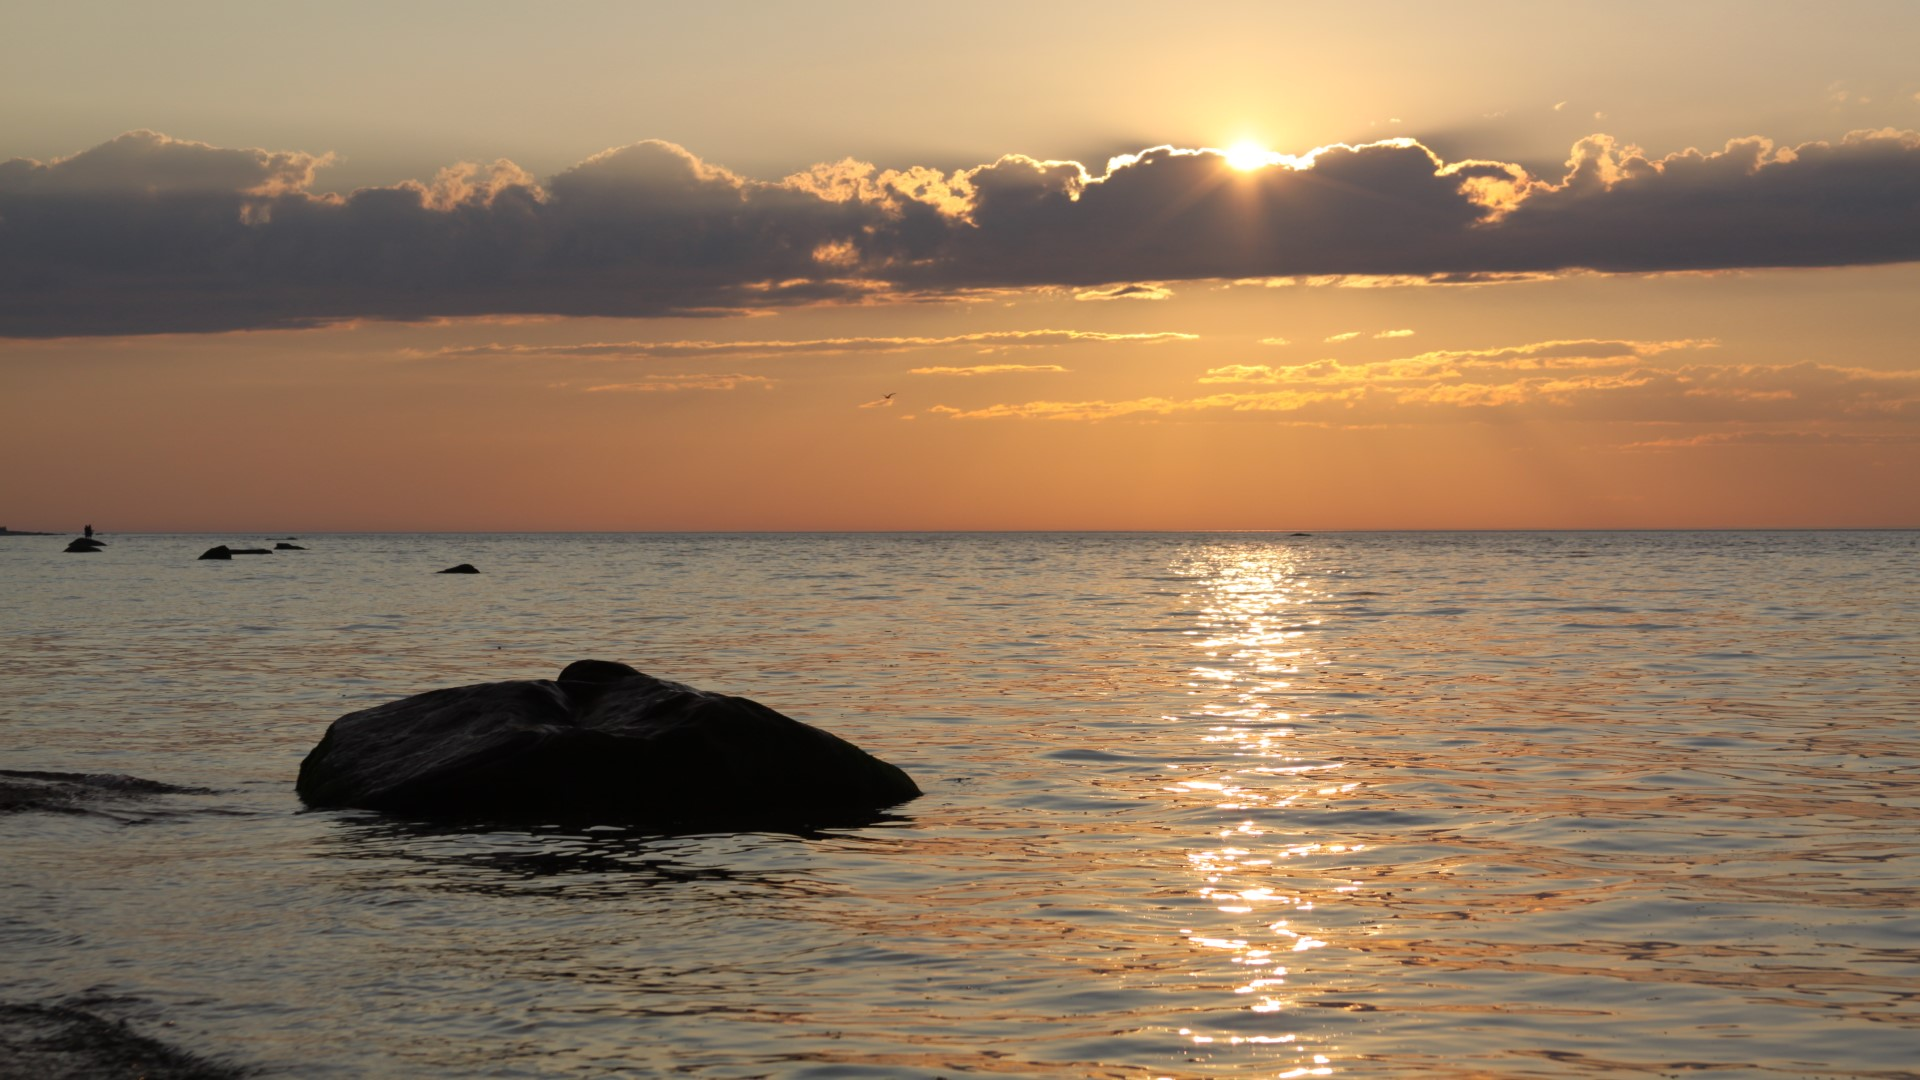
\includegraphics[width = 0.5\textwidth]{demo}
    \caption{"hello there"} %captions required for a referenced figure 
    \label{fig:figure1} %the "fig" is not required but good style 
\end{figure}

%Here is a wrapping environment. The text AFTER the figure will be wrapped around the figure 
\begin{wrapfigure}{r}{0.25\textwidth} %use "l" for left, and "r" for right
    %the size above determines the size of the box
    \centering
    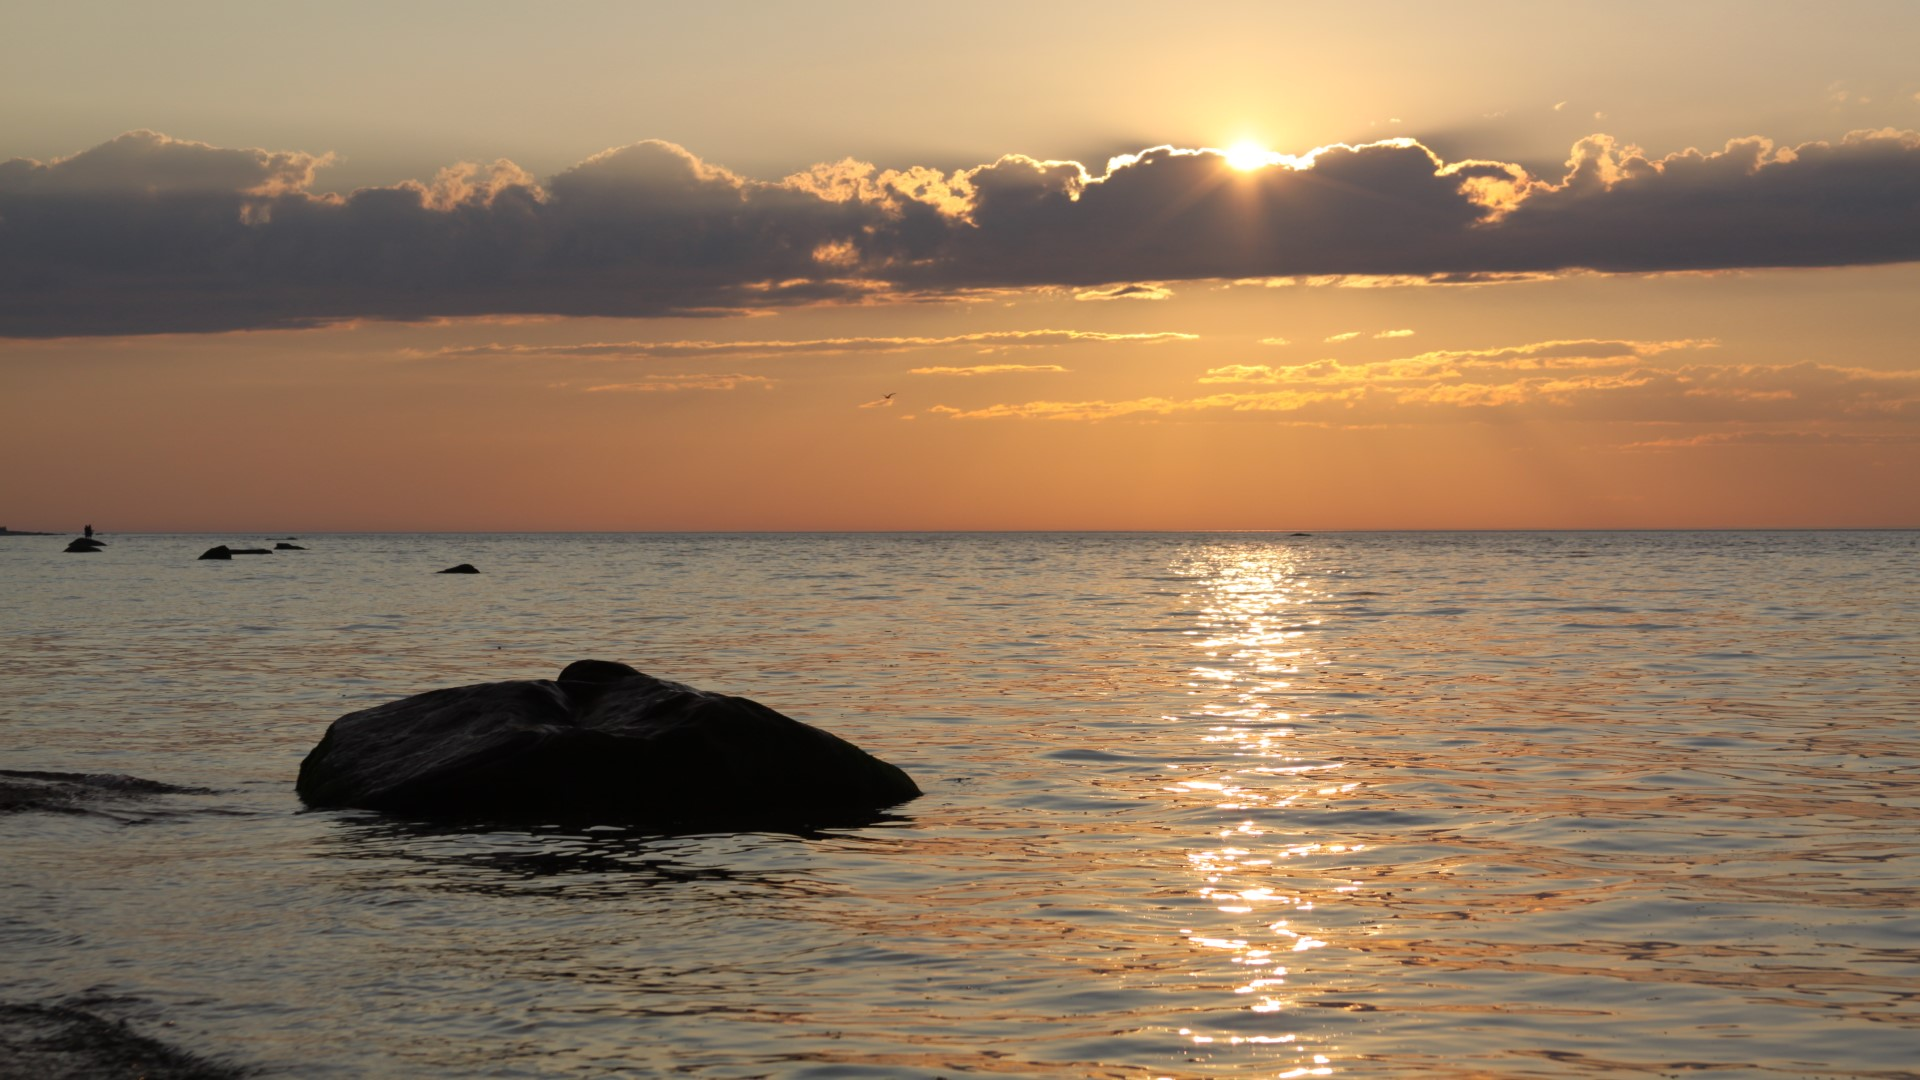
\includegraphics[width = 0.25\textwidth]{demo} %the size here determines the size of the image
\end{wrapfigure}

As you can see in Figure \ref{fig:figure1}, we have an image that is referenceable. This is present on page \pageref{fig:figure1}.  Here is some more text that is designed to wrap around the figure for demonstration purposes. Here is some more text that is designed to wrap around the figure for demonstration purposes. Here is some more text that is designed to wrap around the figure for demonstration purposes. Here is some more text that is designed to wrap around the figure for demonstration purposes. 

%here, we use a right caption 
\begin{SCfigure}[0.5][h] %0.5 means that we take up half of the width for hte caption 
\caption{Here is a right caption!}
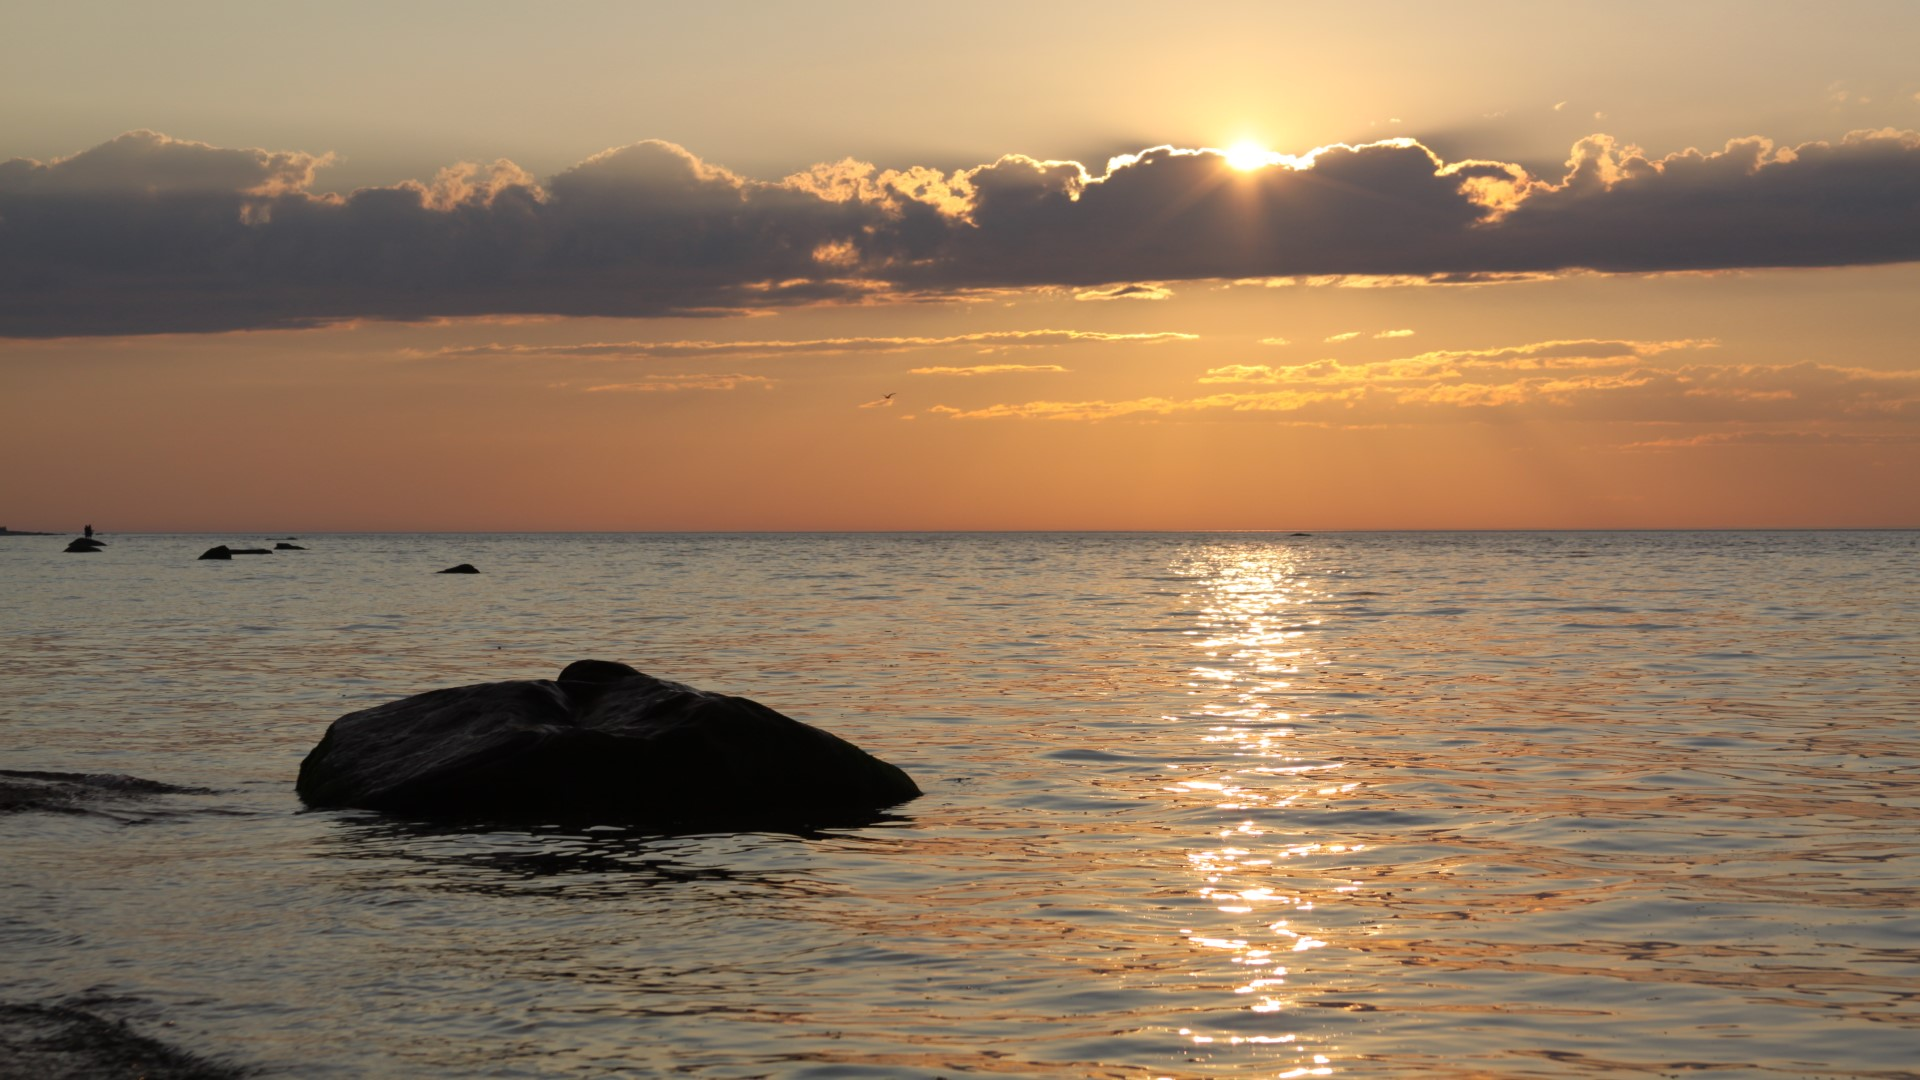
\includegraphics[width=0.6\textwidth]{demo}
\end{SCfigure}

\end{document}